\documentclass{article}[12pt]
\usepackage{fontspec}   %加這個就可以設定字體
\usepackage{xeCJK}       %讓中英文字體分開設置
\usepackage{indentfirst}
\usepackage{listings}
\usepackage[newfloat]{minted}
\usepackage{float}
\usepackage{graphicx}
\usepackage{caption}
\usepackage{fancyhdr}
\usepackage{hyperref}
\usepackage{amsmath}
\usepackage{multirow}
\usepackage[dvipsnames]{xcolor}
\usepackage{graphicx}
\usepackage{tabularx}
\usepackage{booktabs}
\usepackage{caption}
\usepackage{subcaption}
\usepackage{pifont}
\usepackage{amssymb}
\usepackage{titling}

\usepackage{pdftexcmds}
\usepackage{catchfile}
\usepackage{ifluatex}
\usepackage{ifplatform}

\usepackage[breakable, listings, skins, minted]{tcolorbox}
\usepackage{etoolbox}
\setminted{fontsize=\footnotesize}
\renewtcblisting{minted}{%
    listing engine=minted,
    minted language=python,
    listing only,
    breakable,
    enhanced,
    minted options = {
        linenos, 
        breaklines=true, 
        breakbefore=., 
        % fontsize=\footnotesize, 
        numbersep=2mm
    },
    overlay={%
        \begin{tcbclipinterior}
            \fill[gray!25] (frame.south west) rectangle ([xshift=4mm]frame.north west);
        \end{tcbclipinterior}
    }   
}

\usepackage[
top=1.5cm,
bottom=1.5cm,
left=2.5cm,
right=2.5cm,
includehead,includefoot,
heightrounded, % to avoid spurious underfull messages
]{geometry} 

\newenvironment{code}{\captionsetup{type=listing}}{}
\SetupFloatingEnvironment{listing}{name=Code}
\usepackage[moderate]{savetrees}


\title{TCG HW1 Report}
\author{110550088 李杰穎}
\date{\today}


\setCJKmainfont{Noto Serif TC}

\iflinux
\setmonofont[Mapping=tex-text]{Cascadia Code}
\fi

\ifwindows
\setmonofont[Mapping=tex-text]{Consolas}
\fi

\XeTeXlinebreaklocale "zh"             %這兩行一定要加,中文才能自動換行
\XeTeXlinebreakskip = 0pt plus 1pt     %這兩行一定要加,中文才能自動換行

\setlength{\parindent}{0em}
\setlength{\parskip}{2em}
\renewcommand{\baselinestretch}{1.25}
\setlength{\droptitle}{-10em}   % This is your set screw

\begin{document}

\maketitle

\section{Question 1}

In this question, we assume that the 2048 game ends when any of tiles reach 2048.

\subsection{State-space Complexity}
First, each tiles can be empty, 2, 4, 8, 16, 32, 64, ..., 1024, in total 12 possibilities, and the game has 16 tiles. Therefore, the state-space complexity is ${12}^{16} \approx 1.85 \times {10}^{17}$.

\subsection{Game-tree Complexity}

Because 2048 is quite random, we can only estimate a loose upper bound. Below are the needed assumptions to estimate the upper bound of game-tree complexity.

\begin{enumerate}
	\item We can always perform 4 legal moves, that is up, down, right and left.
	\item There always have 15 tiles that can generate new tile.
	\item A generated tiles will always be 2. 4 won't be generated. This can calculate a looser upper bound.
	\item If the total sum of tiles on the board reaches 2048, we will immediately combine those tiles to get a 2048 tiles and the game ends. The maximum steps to combine all the tiles is 10 steps, because $2 \rightarrow 4 \rightarrow 8 \rightarrow \cdots \rightarrow 2048$ in total 10 steps.
	\item Don't consider duplicate board.
\end{enumerate}

By the assumptions above, to reach 2048, we need to generate $\frac{2048}{2} = 1024$ tiles. And there are two randomly placed tiles at the beginning of the game, so to reach the sum of all tiles equals to 2048, we need $1022$ moves. 

In each moves, we can choose one direction out of 4 choices, and a tiles will be placed on one of the 15 tiles. This tiles can be a 2 or 4 (This doesn't violate the assumption, because we want to have a looser upper bound). Therefore, in each move we have $4 \times 30 = 120$ possible outcomes.

Therefore, the upper bound of game-tree complexity is $120^{1022+10} \approx 5.19 \times 10^{2145}$.

\section{Question 2}

We know that the longer side always win the game using the mirror strategy, below is the proof.

First, we assume that A (the longer side) is white, because if A is black it will have more advantages. Therefore, if we can prove that A always win even when it is white, then it will also always win when it's black. Because being black is no worse than white.

Second, WLOG, we can first look at the 4 hexes enclosed by the red line. If B cross the split line via R to O, then we will find that B can't never win the game, because the route the another side has already blocked by A. 

\begin{figure}[H]
	\centering
	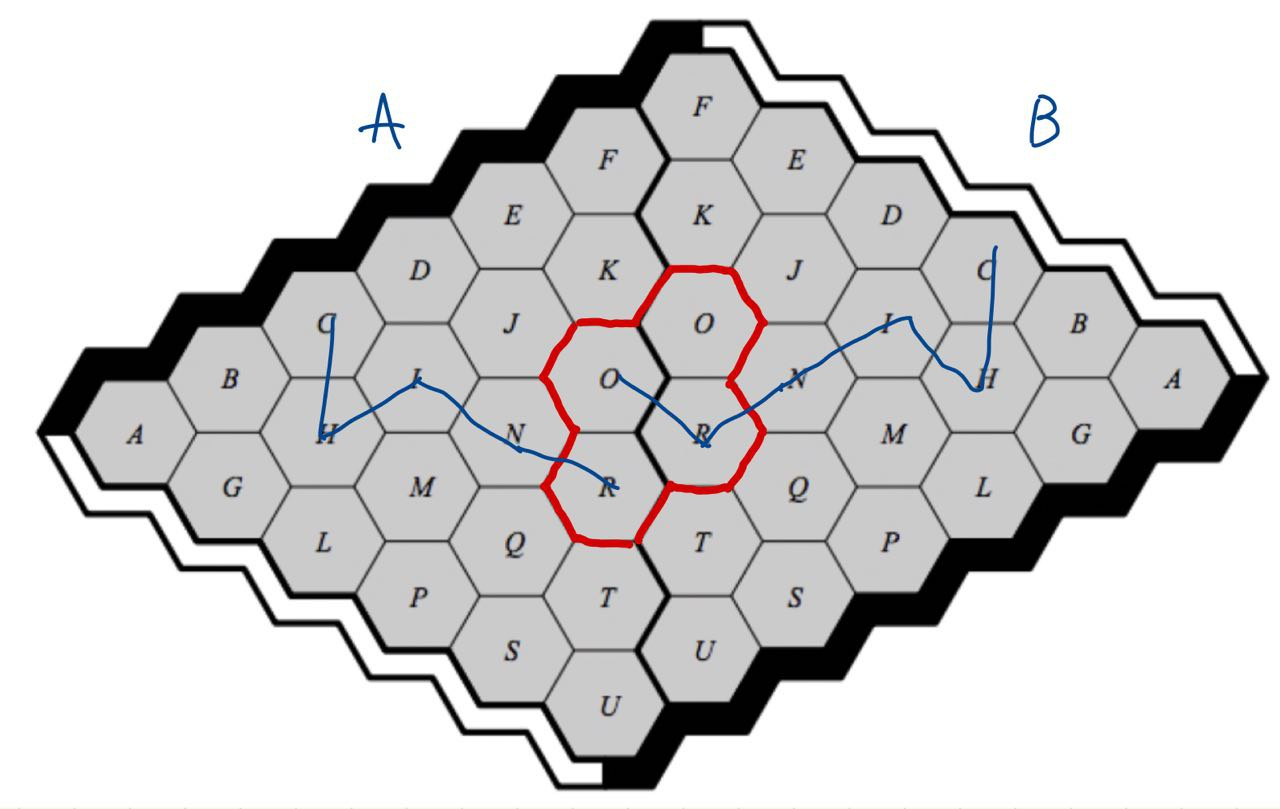
\includegraphics[width=0.7\linewidth]{hex}
	\caption{This figure shows that A (the longer side) always win the hex game no matter it is black or white using the mirror strategy.}
	\label{fig:hex}
\end{figure}


\section{Question 3}

For $\text{Connect}(m,\ n,\ k,\ p,\ q+1)$, black can first play additional chess arbitrary, and follow the optimal strategy of $\text{Connect}(m,\ n,\ k,\ p,\ q)$. If the optimal strategy places the chess on the previous placed chess, just placed another chess arbitrary. In conclusion, because the additional chess won't harm black, $\text{Connect}(m,\ n,\ k,\ p,\ q+1)$ for Black is no worse than that in $\text{Connect}(m,\ n,\ k,\ p,\ q)$.

\section{Question 4}

Connect$(6, \ 2, \ 2)$ and Hex can be both ultra-weakly solved with no win for White by strategy-stealing. 

We first look at (b), (c) and (e), we can notice that if we swap color of black and white, the board will all be identical before swapping, thus, we can use same technique, which is strategy-stealing to prove that (b), (c) and (e) can be solved ultra-weakly.

For (a) and (d), after swapping color, the board is different, so we can't use strategy-stealing. In conclusion, I think it's impossible to prove that (a) and (d) can be solved ultra-weakly.


\end{document}